\documentclass{beamer}
\usepackage{multimedia}
\usepackage{soul}
\usepackage{amsmath}
\usepackage{transparent}






\usetheme{Warsaw}
\setbeamertemplate{navigation symbols}{}

\title{SHOCKWAVE}
\author{Max L$\hat{\textrm{e}}$}
% \titlegraphic{\transparent{0.4}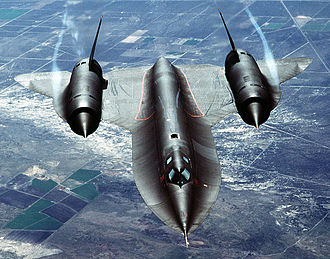
\includegraphics[width=40mm,height=40mm]{sr71.jpg}{\centering}}
\begin{document}




    {
    \usebackgroundtemplate{\transparent{0.2}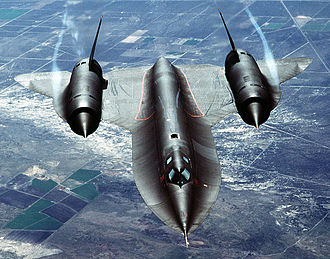
\includegraphics[width=\paperwidth]{sr71.jpg}}
    \begin{frame}
        \maketitle
    \end{frame}
    }

    \section{OVERVIEW}    
    \begin{frame}
        \frametitle{Overview}
        \begin{itemize}
            \item Problem Statement 
            \item Methods 
            \item Results
            \item Conclusions
            \item Q\&A            
        \end{itemize}
    \end{frame}
    
    \section{PROBLEM STATEMENT}
    \begin{frame}
        \frametitle{Motivation}
        \begin{columns}
        \column{.5\textwidth}
        \begin{figure}
            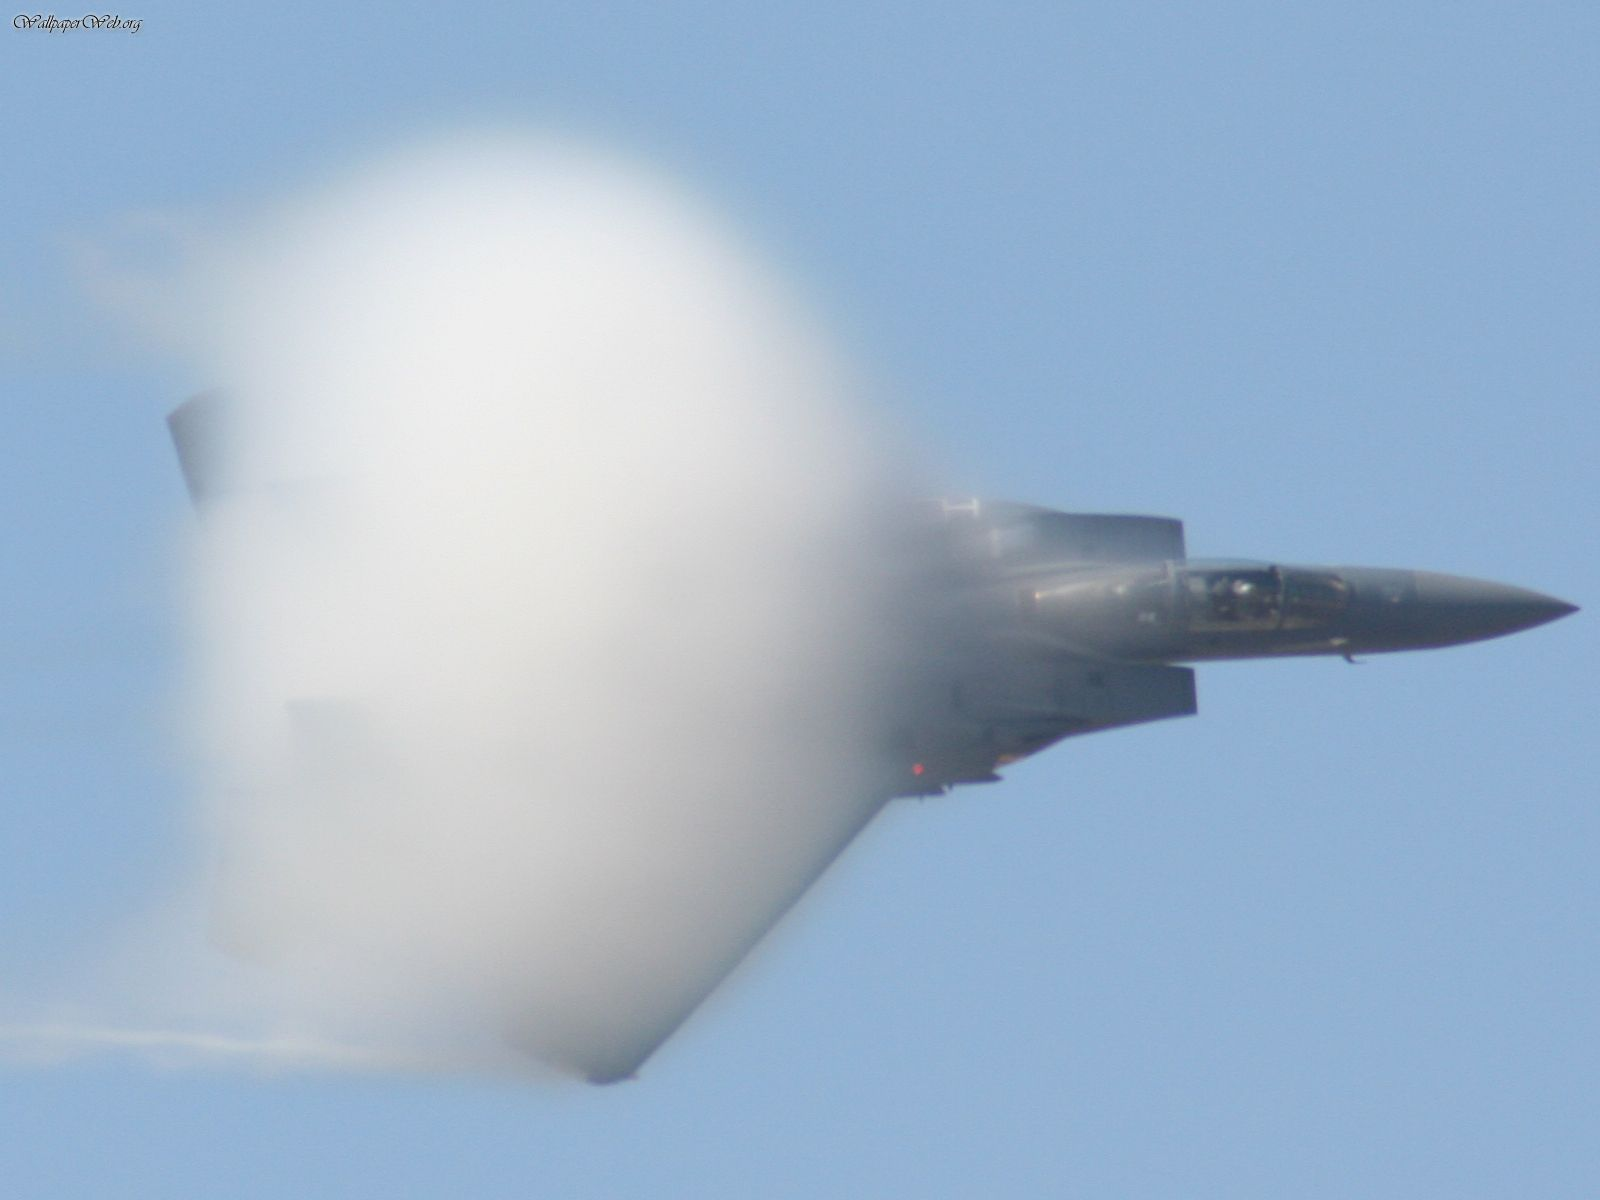
\includegraphics[height = 30mm,width = 50mm]{f15shock.JPG}
            \caption{Shock cloud F15}
        \end{figure}
        

        \column{.5\textwidth}
        \begin{itemize}
            \item Shockwaves are important in aerodynamics
            \item In aircraft: when approach speed of sound 
            \item In detonation: blast wave causes very dangerous shock
            \item Across shocks, properties are chaotic $\rightarrow$ Need good shock capturing schemes            
        \end{itemize}
        \end{columns}        
    \end{frame}

    \begin{frame}
        \frametitle{The Shocktube}
        \begin{columns}
            \column{.5\textwidth}
            \begin{figure}
                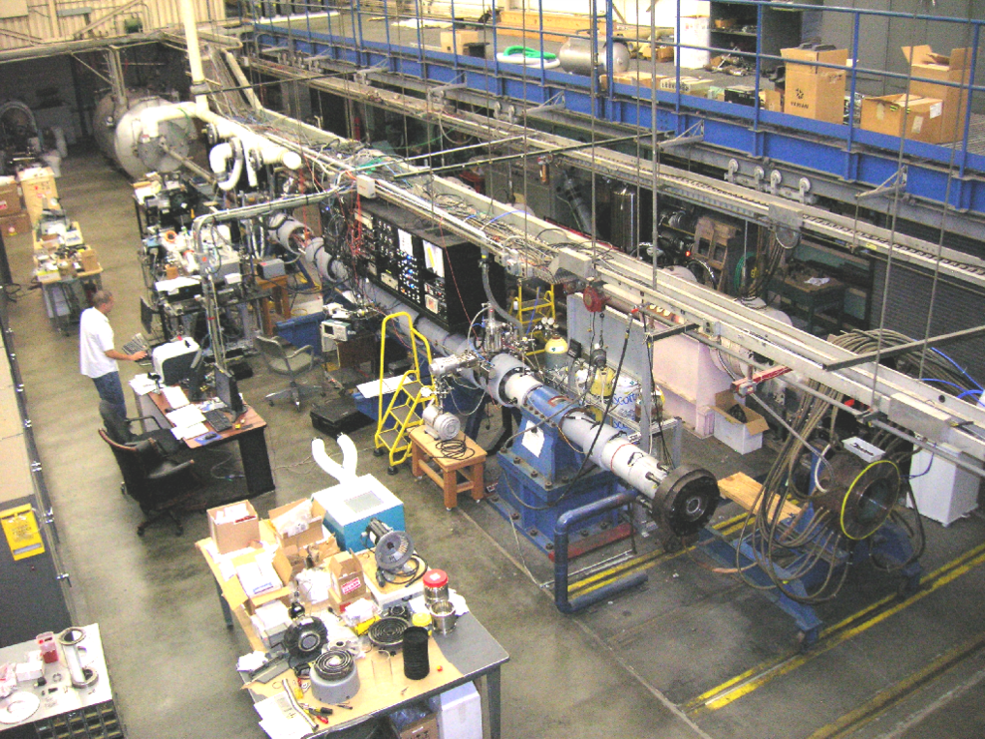
\includegraphics[height = 30mm,width = 50mm]{nasa_shocktube.png}
                \caption{NASA Ames 9m shocktube}
            \end{figure}
    
            \column{.5\textwidth}
            \begin{itemize}
                \item simple mechanical device with low and high properties at both end
                \item A diaphragm separates the two fluid. 
                \item Once diaphgragm breaks, \textbf{shockwave} propagates to the right, expansion wave propagates to the left
            \end{itemize}
            \end{columns}        
    \end{frame}


    \begin{frame}
        \frametitle{The Shocktube}       
            \begin{figure}
                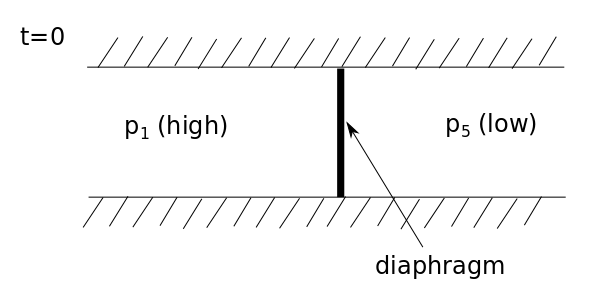
\includegraphics[height = 40mm,width = 80mm]{IC_sod.png}
                \caption{Initial conditions}
            \end{figure}          
    \end{frame}


    \begin{frame}
        \frametitle{The Shocktube}       
            \begin{figure}
                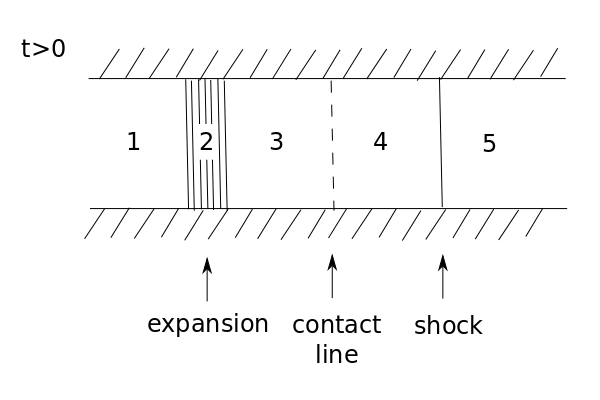
\includegraphics[height = 40mm,width = 80mm]{solution_sod.png}
                \caption{After diaphragm breaks}
            \end{figure}          
    \end{frame}


    \begin{frame}
        \frametitle{Assumptions}
        \begin{itemize}
            \item Ideal gas 
            \item Single phase flow
            \item Zero gradient boundary conditions at both ends
            \item No heat transfer, no body force
            \item \st{Incompressible}
            \item \st{Steady State}        
        \end{itemize}        
    \end{frame}

    \begin{frame}
        \frametitle{Equations}
        \begin{columns}
        \column{.5\textwidth}
        \begin{figure}
            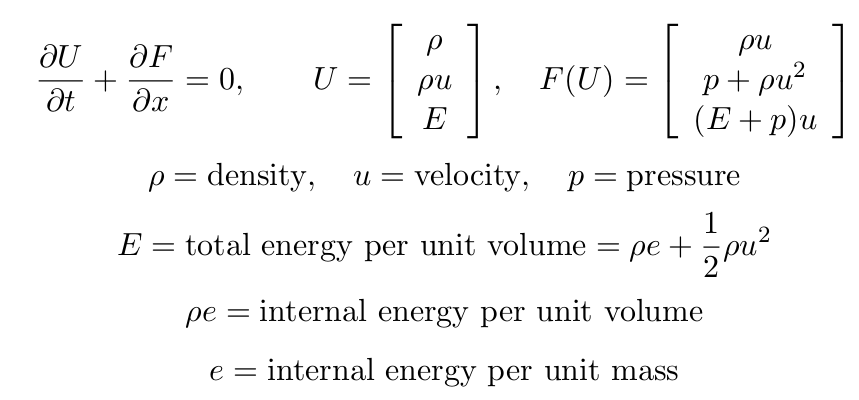
\includegraphics[height = 40mm,width = 50mm]{euler1d.jpg}
        \end{figure}

        \column{.5\textwidth}
        \begin{itemize}
            \item Conservation of mass,momentum and energy
            \item Ideal gas equation of state to close the system 
        \end{itemize}
        \end{columns}        
    \end{frame}

    

    \section{METHODS}
    \begin{frame}
        \frametitle{Computational Grid}
        \begin{columns}
            \column{.5\textwidth}
            \begin{figure}
                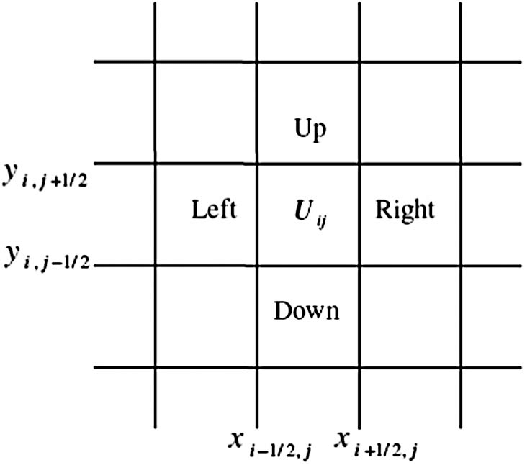
\includegraphics[height = 40mm,width = 50mm]{grid.png}
            \end{figure}   
    
            \column{.5\textwidth}
            \begin{itemize}
                \item Properties at cell's center 
                \item Fluxes on the edge
            \end{itemize}
            \end{columns}        
    \end{frame}

    \begin{frame}
        \frametitle{Numerical Schemes}
        \begin{columns}
            \column{.5\textwidth}
            \begin{align*}
               \dfrac{\partial U}{\partial t} \approx \dfrac{U_i^{n+1}-U_i^n}{\Delta t} + \mathcal{O}(\Delta t)\\
            \end{align*}

            \begin{align*}
                \dfrac{\partial F}{\partial x} \approx \dfrac{F_{i+1}^{n1}-F_{i}^n}{\Delta x} + \mathcal{O}(\Delta x)\\
            \end{align*}


    
            \column{.5\textwidth}
            \begin{itemize}
                \item Temporal discretization: first order forward in time 
                \item Spatial discretization: first order in space
                \item Fluxes are calculated as \textbf{Van Leer} fluxes for subsonic and supersonic case. 
            \end{itemize}
            \end{columns}        
    \end{frame}



    \begin{frame}
        \frametitle{Numerical Schemes}
        \begin{equation*}
            U^{n+1}_{i} = U_i^n-\dfrac{\Delta t}{\Delta x}\left[(F^+ + F^-)_{i+1/2}-(F^+ + F^-)_{i-1/2}\right]
        \end{equation*}        
    \end{frame}

    

    \begin{frame}
        \frametitle{Parallelization Strategy}
            \begin{figure}
                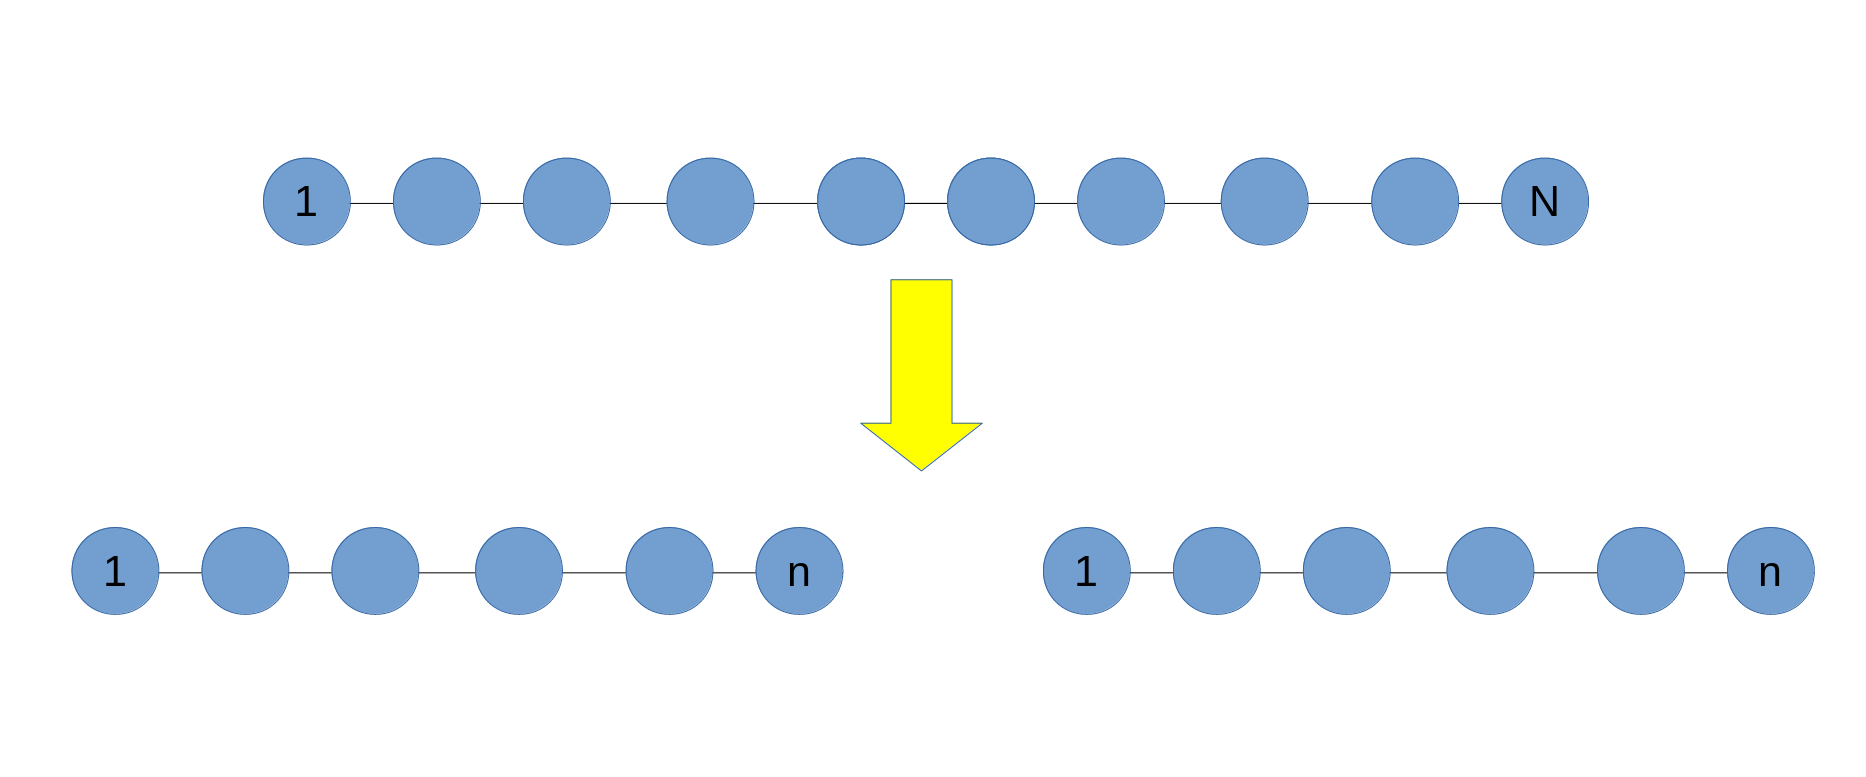
\includegraphics[height = 40mm,width = 100mm]{split.png}                
            \end{figure}        
    \end{frame}

    \begin{frame}
        \frametitle{Optimizations}
            \begin{figure}
                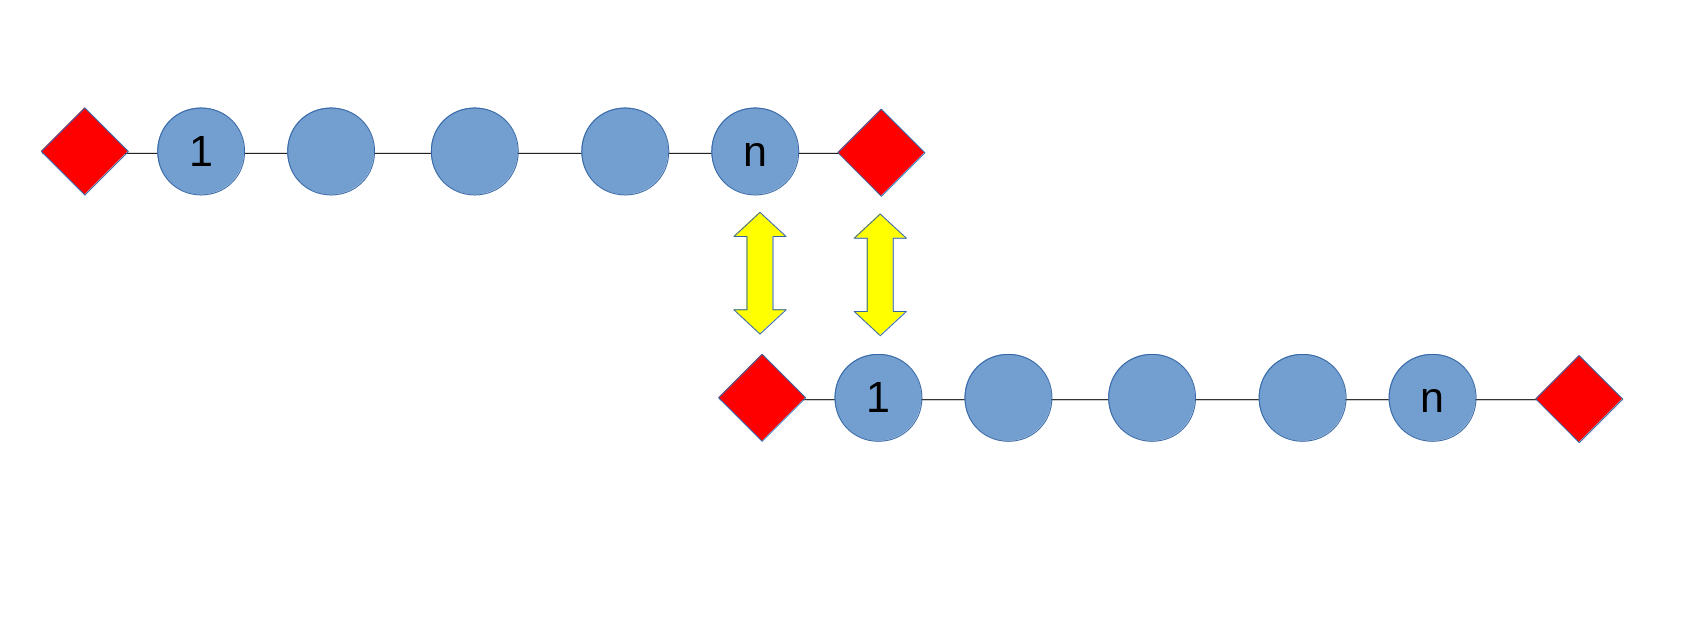
\includegraphics[height = 40mm,width = 100mm]{ghost.png}                
            \end{figure}        
    \end{frame}

    \section{RESULTS}

    \begin{frame}
        \frametitle{Numerical evolutions}
            \begin{figure}
                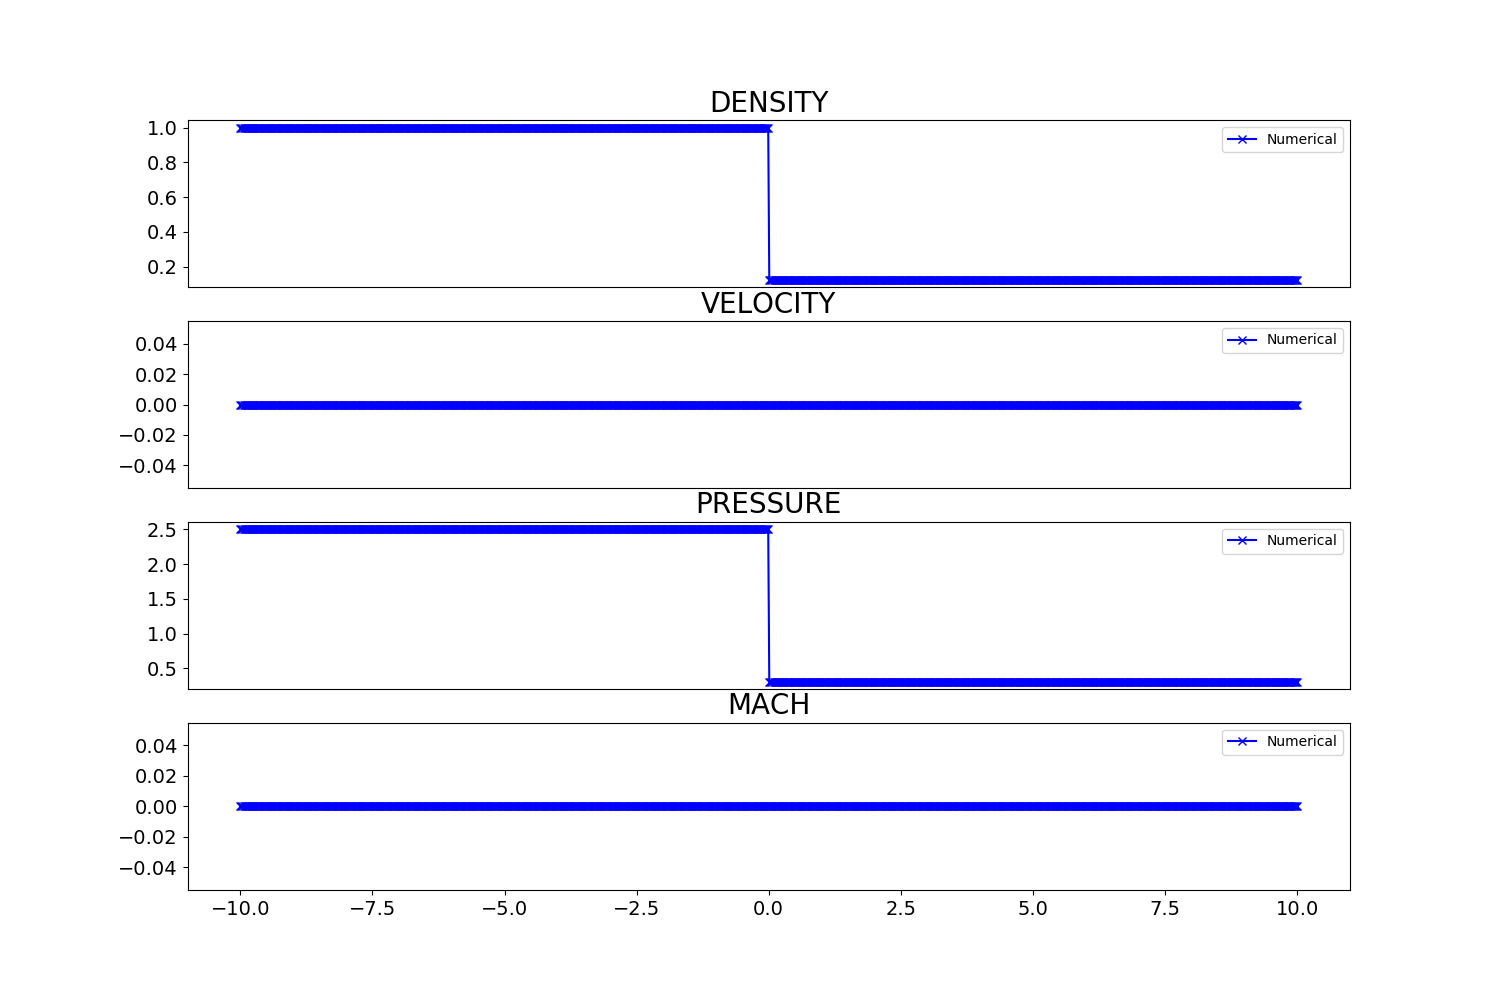
\includegraphics[height = 60mm,width = 100mm]{shock0.png}             
            \end{figure}        
    \end{frame}
    

    \begin{frame}
        \frametitle{Numerical evolutions}
            \begin{figure}
                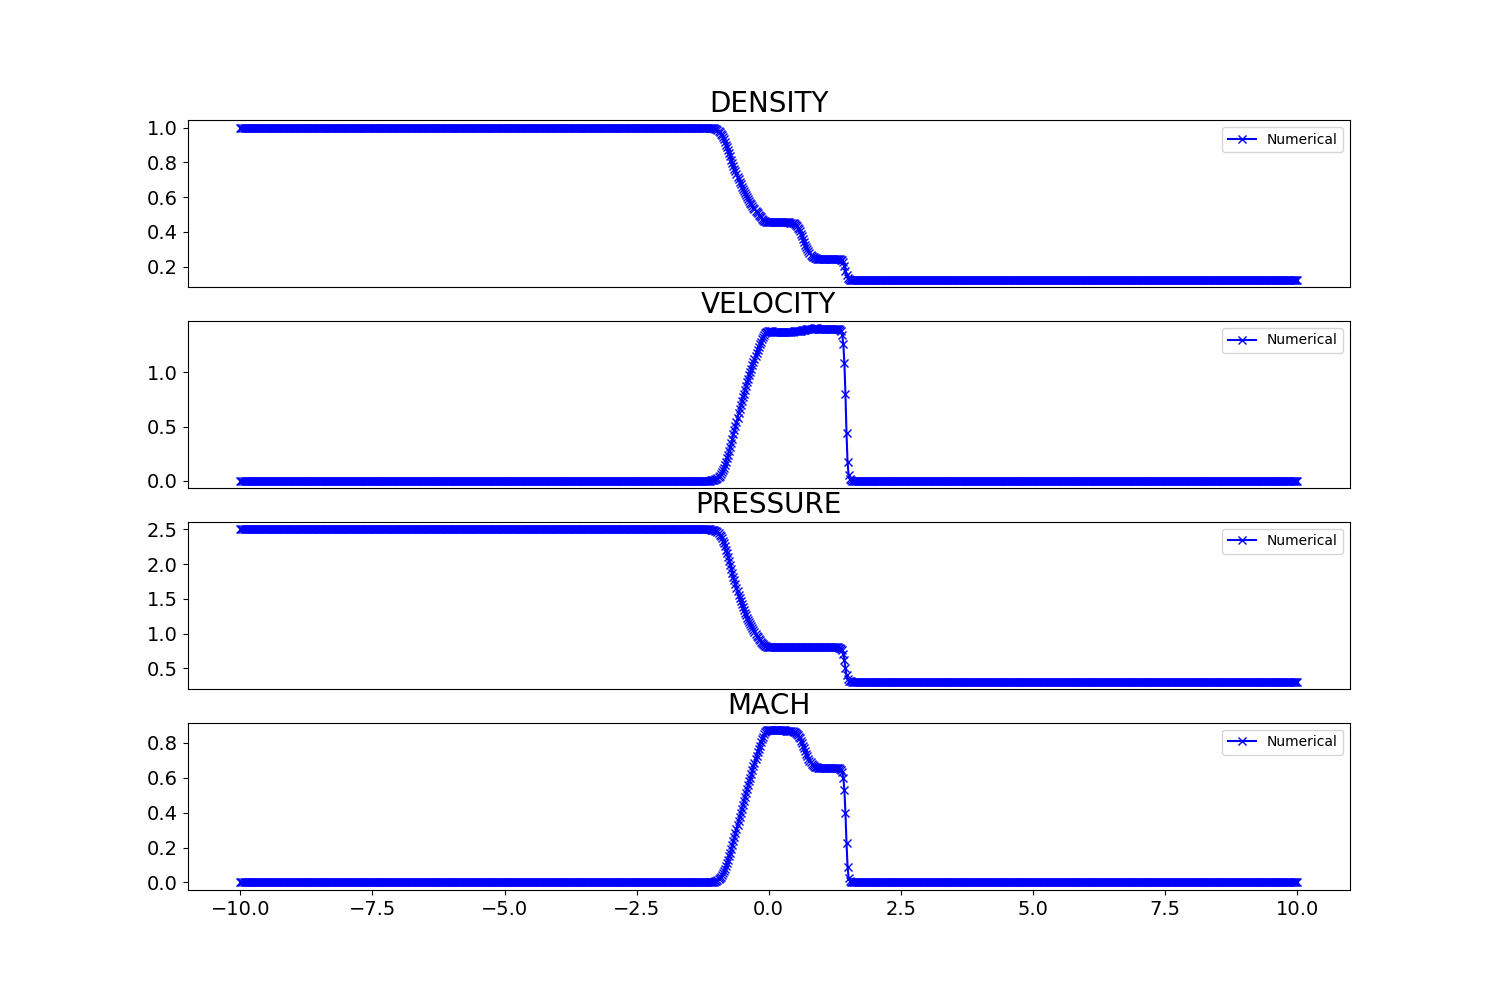
\includegraphics[height = 60mm,width = 100mm]{shock2.png}             
            \end{figure}        
    \end{frame}

    \begin{frame}
        \frametitle{Numerical evolutions}
            \begin{figure}
                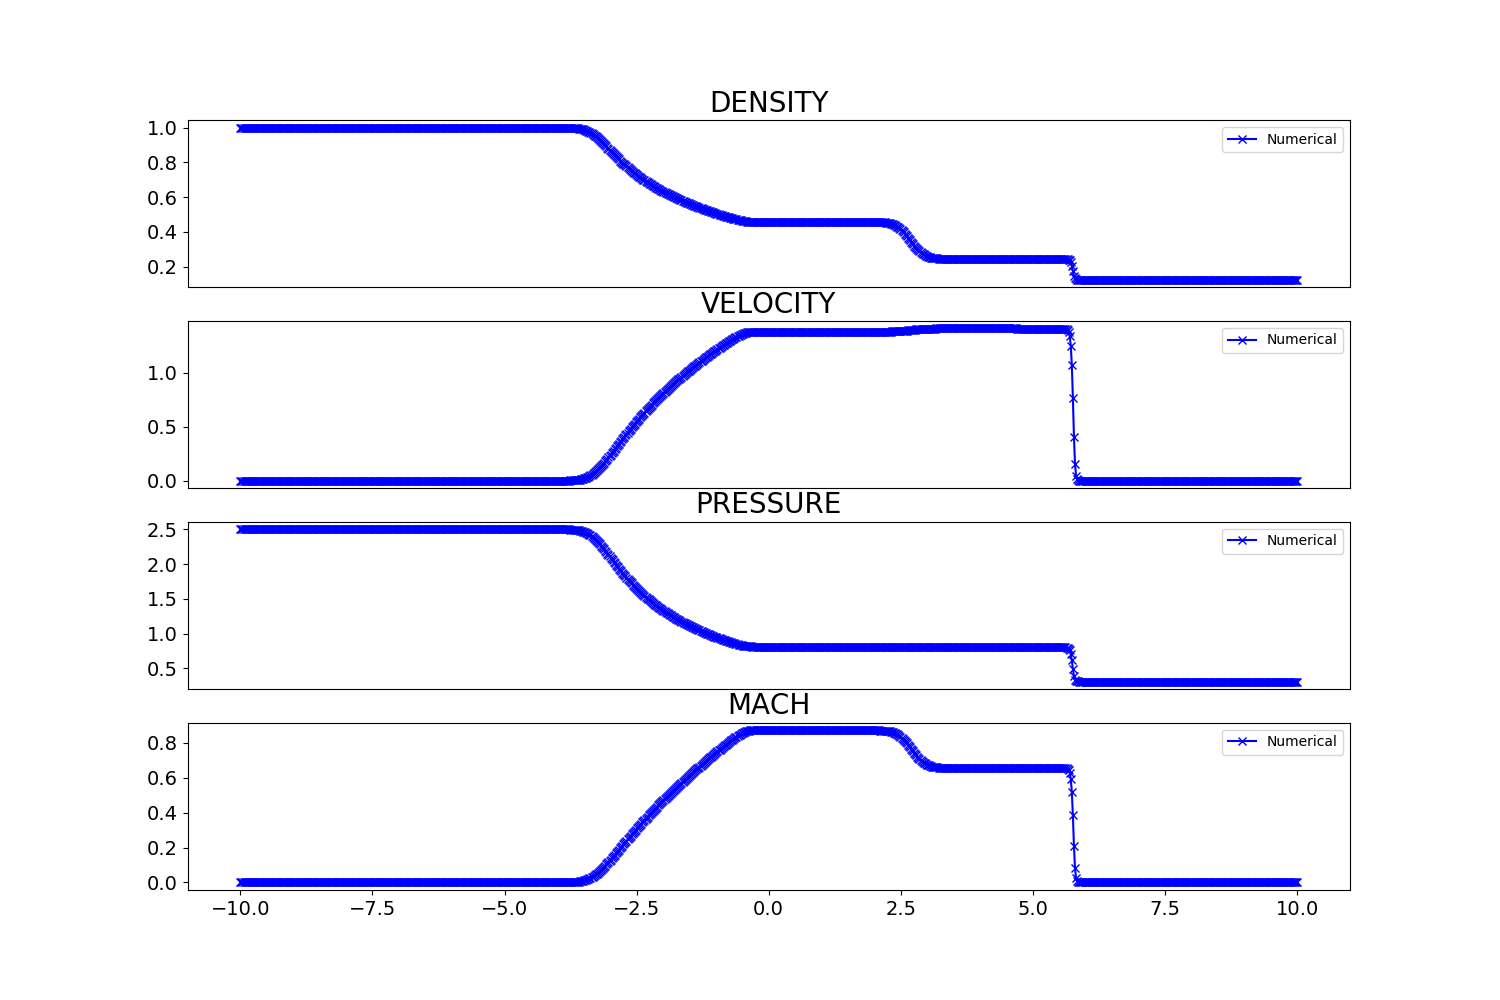
\includegraphics[height = 60mm,width = 100mm]{shock3.png}             
            \end{figure}        
    \end{frame}


    \begin{frame}
        \frametitle{Analytical comparison}
            \begin{figure}
                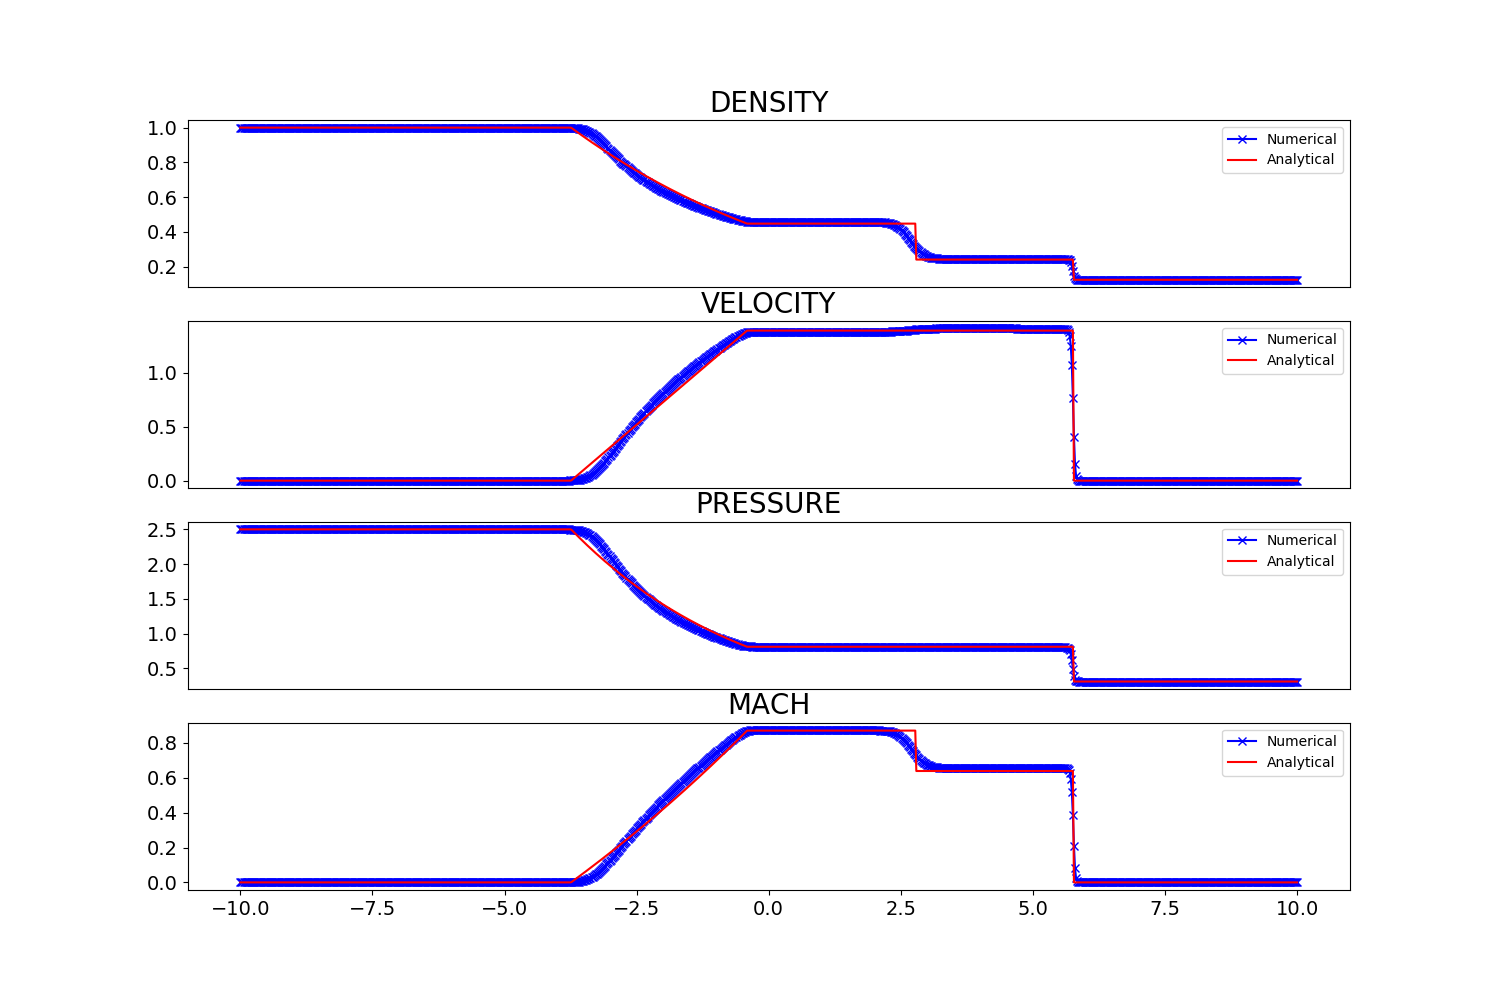
\includegraphics[height = 60mm,width = 100mm]{ana_num.png}             
            \end{figure}            
    \end{frame}

    \begin{frame}
        \frametitle{Speedup}
        
        \begin{columns}
            \column{0.5\textwidth}
            \begin{figure}
                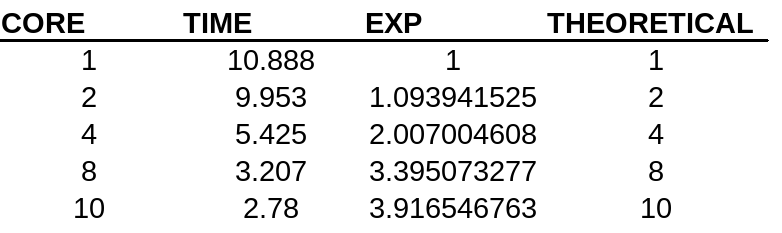
\includegraphics[height = 20mm,width = 50mm]{table_1g_speed.png}             
            \end{figure}       
    
            \column{.5\textwidth}
            \begin{figure}
                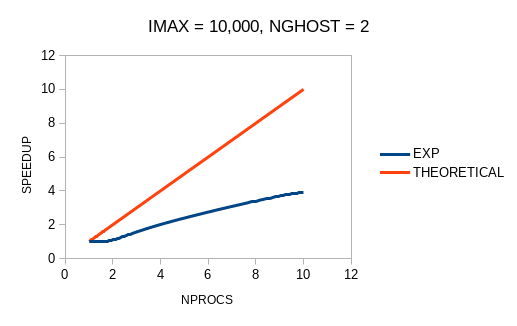
\includegraphics[height = 40mm,width = 50mm]{plot_1g_speed.png}            
            \end{figure}       
            \end{columns}
    \end{frame}

    \begin{frame}
        \frametitle{Ghost Points}
        
        \begin{columns}
            \column{0.5\textwidth}
            \begin{figure}
                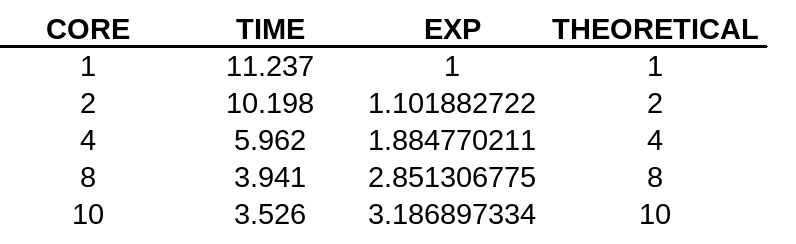
\includegraphics[height = 20mm,width = 50mm]{table_10g_speed.png}             
            \end{figure}       
    
            \column{.5\textwidth}
            \begin{figure}
                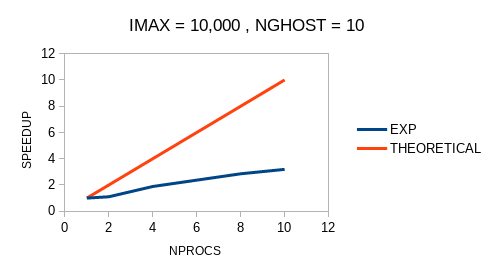
\includegraphics[height = 40mm,width = 50mm]{plot_10g_speed.png}            
            \end{figure}       
            \end{columns}

    \end{frame}

    \begin{frame}
        \frametitle{Scaling}
        
        \begin{columns}
            \column{0.5\textwidth}
            \begin{figure}
                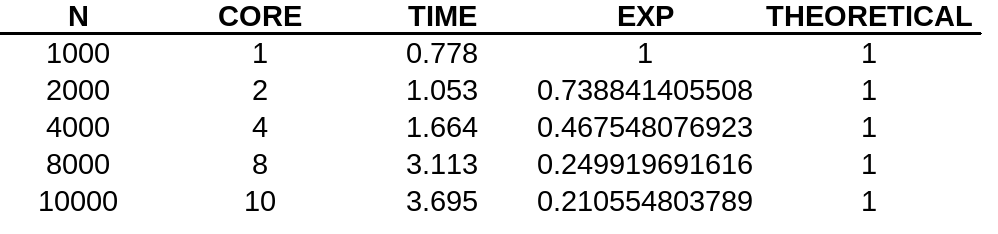
\includegraphics[height = 15mm,width = 50mm]{scaleBStable.png}             
            \end{figure}       
    
            \column{.5\textwidth}
            \begin{figure}
                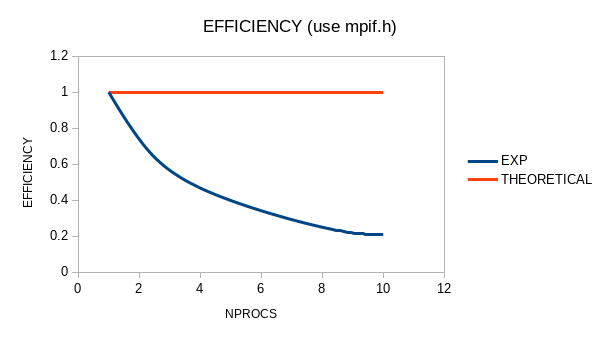
\includegraphics[height = 40mm,width = 50mm]{scaleBSplot.png}            
            \end{figure}       
            \end{columns}
    \end{frame}


    \begin{frame}
        \frametitle{Scaling}
        
        \begin{columns}
            \column{0.5\textwidth}
            \begin{figure}
                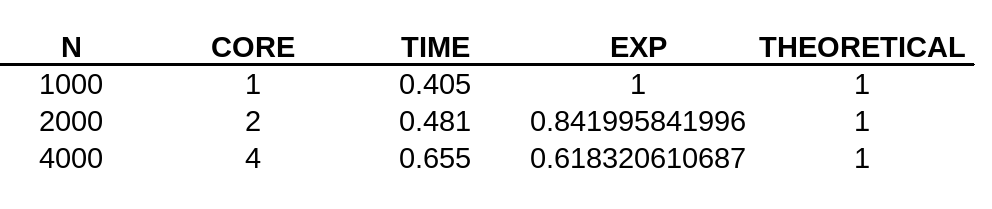
\includegraphics[height = 15mm,width = 50mm]{scaleMPItable.png}             
            \end{figure}       
    
            \column{.5\textwidth}
            \begin{figure}
                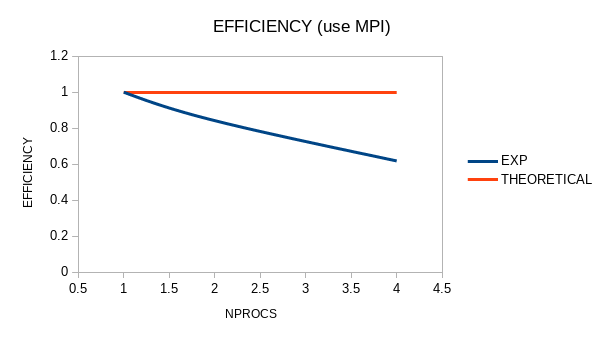
\includegraphics[height = 40mm,width = 50mm]{scaleMPIplot.png}       
            \end{figure}       
            \end{columns}
    \end{frame}



    \section{CONCLUSIONS}
    \begin{frame}
        \frametitle{Some remarks}
        \begin{itemize}
            \item We do see speedup but not great 
            \item Extended ghost layers do not give much speedup 
            \item Improvements: solve cons of mass, momentum, energy individually (instead of grouping everything under 1 U state vector) $\Rightarrow$ need individual fluxes
        \end{itemize}      

    \end{frame}


    \begin{frame}
        \frametitle{References}
        \begin{itemize}
            \item MTH/CSE 4280 Parallel Process Lecture Notes
            \item Chimera CFD . Van Leer Flux Splitting Scheme.
            \item AEE 5350 CFD Lecture Notes 
            
        \end{itemize}
        
    \end{frame}

    \begin{frame}
        \begin{center}
            \noindent
            \Large{Thank You For Listening! \\ \textit{(Remember: Go with with the flow)}}
            
        \end{center}
    \end{frame}

    



    







\end{document}